\documentclass[a4paper, 11pt]{article}\usepackage[]{graphicx}\usepackage[]{xcolor}
% maxwidth is the original width if it is less than linewidth
% otherwise use linewidth (to make sure the graphics do not exceed the margin)
\makeatletter
\def\maxwidth{ %
  \ifdim\Gin@nat@width>\linewidth
    \linewidth
  \else
    \Gin@nat@width
  \fi
}
\makeatother

\definecolor{fgcolor}{rgb}{0.345, 0.345, 0.345}
\newcommand{\hlnum}[1]{\textcolor[rgb]{0.686,0.059,0.569}{#1}}%
\newcommand{\hlstr}[1]{\textcolor[rgb]{0.192,0.494,0.8}{#1}}%
\newcommand{\hlcom}[1]{\textcolor[rgb]{0.678,0.584,0.686}{\textit{#1}}}%
\newcommand{\hlopt}[1]{\textcolor[rgb]{0,0,0}{#1}}%
\newcommand{\hlstd}[1]{\textcolor[rgb]{0.345,0.345,0.345}{#1}}%
\newcommand{\hlkwa}[1]{\textcolor[rgb]{0.161,0.373,0.58}{\textbf{#1}}}%
\newcommand{\hlkwb}[1]{\textcolor[rgb]{0.69,0.353,0.396}{#1}}%
\newcommand{\hlkwc}[1]{\textcolor[rgb]{0.333,0.667,0.333}{#1}}%
\newcommand{\hlkwd}[1]{\textcolor[rgb]{0.737,0.353,0.396}{\textbf{#1}}}%
\let\hlipl\hlkwb

\usepackage{framed}
\makeatletter
\newenvironment{kframe}{%
 \def\at@end@of@kframe{}%
 \ifinner\ifhmode%
  \def\at@end@of@kframe{\end{minipage}}%
  \begin{minipage}{\columnwidth}%
 \fi\fi%
 \def\FrameCommand##1{\hskip\@totalleftmargin \hskip-\fboxsep
 \colorbox{shadecolor}{##1}\hskip-\fboxsep
     % There is no \\@totalrightmargin, so:
     \hskip-\linewidth \hskip-\@totalleftmargin \hskip\columnwidth}%
 \MakeFramed {\advance\hsize-\width
   \@totalleftmargin\z@ \linewidth\hsize
   \@setminipage}}%
 {\par\unskip\endMakeFramed%
 \at@end@of@kframe}
\makeatother

\definecolor{shadecolor}{rgb}{.97, .97, .97}
\definecolor{messagecolor}{rgb}{0, 0, 0}
\definecolor{warningcolor}{rgb}{1, 0, 1}
\definecolor{errorcolor}{rgb}{1, 0, 0}
\newenvironment{knitrout}{}{} % an empty environment to be redefined in TeX

\usepackage{alltt}
% package accents
\usepackage[utf8]{inputenc}% input en utf8
\usepackage[french]{babel}% typo française
\usepackage[T1]{fontenc}% accents out en format T1

% package maths
\usepackage{amsmath}
\usepackage{mathtools}
\usepackage{amsfonts}
\usepackage{amssymb}
\usepackage{mathabx}
\usepackage{cases}

% biblio
\usepackage[bibstyle=verbose, citestyle=verbose-trad1, backend=biber, isbn=false, url=false, doi=false]{biblatex}
\bibliography{Biblio.bib}
\DeclareNameAlias{sortname}{family-given} % nom de famille en premier

% mise en forme des paragraphes
\usepackage{parskip}% saut de lignes en fin de paragraphe
\let\EndItemize\enditemize
\def\enditemize{\EndItemize\bigskip}% sauts de ligne en fin d'environnement itemize

% tables et figures
\usepackage{multirow} % permet de fusionner les colonnes
\usepackage{graphicx} % admet les figures
\usepackage{array} % types particuliers de tableaux
\usepackage{tabularx} % autres tableaux, notamment pour gérer les doubles traits de séparation (voir hhline)
\usepackage[hang,small]{caption} % mise en forme du caption

% lignes de code
\usepackage{minted}
\usepackage{listings}  % pour les chunk
\setminted{breaklines} % pour sauter des lignes
\definecolor{bg}{rgb}{0.95,0.95,0.95}

\usepackage{csquotes}% typo française (guillermets)

% mise en page
\usepackage{hyperref} % liens hypertextes
\usepackage[bottom]{footmisc} % mise en forme des notes de bas de page "\footnote"
\usepackage[left=2cm,right=2cm,top=2cm,bottom=2cm]{geometry} % marges

% page de garde/titre (en fonction de la classe de document)
\usepackage{titling} % pour le titre en gras
\author{\href{mailto:julioricardo.davalos@ehess.fr}{Julio Ricardo Davalos}}
\title{Petite introduction à \LaTeX{} en Sciences Sociales}
\date{Septembre 2022}

% pour tableaux stargazer et kable
\usepackage{dcolumn}
\usepackage{rotating}
\usepackage{graphicx}
\usepackage{xstring}
\usepackage{array} 
\usepackage{tabularx}
\usepackage{multirow}
\usepackage{booktabs}

% macros
\newcommand{\etoiles}{%
	\begin{center}
    $\ast$\\ $\ast$~\hspace*{2mm}~$\ast$\\
  \end{center}
}
\newcommand{\nomfonction}[2][]{\texttt{\textbackslash#2\{#1\}}}

%-------------------------------Options pour Sweave--------------------------------


\IfFileExists{upquote.sty}{\usepackage{upquote}}{}
\begin{document}

\maketitle

\section*{Introduction}
Ce document a pour but d'introduire à l'utilisation du langage \LaTeX{} à un public venant des SHS. En effet, ce langage est assez commun dans les sciences expérimentales mais reste inconnu (ou alors connu que de nom) pour beaucoup de chercheurs et étudiants en SHS. Cela peut être dû à son côté austère ou encore au fait qu'il peut paraître destiné uniquement à réaliser de belles équations -- capacité que l'on peut considérer comme secondaire voire superflue en SHS.

\subsection*{C'est quoi \LaTeX ?}
\LaTeX{} est un système de composition de document qui permet de produire une mise en page la plus proche possible des normes typographiques d'une langue donnée. Ce système permet de se concentrer sur le fond et le contenu du document à produire en automatisant sa forme. Il fonctionne généralement dans un éditeur de texte -- \TeX maker par exemple mais il en existe bien d'autres -- dans lequel on écrit l'ensemble des commandes qui paramètrent le document avant de le compiler. 

Un éditeur de texte n'est pas un traitement de texte, ce dernier comprenant la mise en forme alors que l'éditeur contient des lignes de code. L'exemple le plus connu des éditeurs est le bloc-note de Windows. Il comprend donc le texte brut que l'on veut éditer et de potentielles commandes informatiques qui formatent leur aspect dans le document final. Le traitement de texte doit donc en permanence rafraîchir la mise en forme du texte afin de montrer en même temps ce que l'on est en train d'écrire et le rendu final, là où l'éditeur ne montre que les lignes de code et ne montrerait le rendu final que s'il comprend un compilateur.

\subsection*{Mais quel est l'intérêt de l'utilisation de \LaTeX ?}
Beaucoup d'arguments sont énoncés concernant les gains à l'utilisation de \LaTeX{} notamment par rapport à un traitement de texte du type Word, j'en retiens les principales qui pourraient retenir l'attention pour une utilisation en SHS.

Comme dit plus haut, il est utilisé pour ses équations et cela peut paraître comme sa seule utilité. Pourtant, il s'agit avant tout d'un langage permettant \emph{une mise en page harmonieuse}, ce qui est fortement requis dans un champs où l'on a tendance à beaucoup écrire. Débarrassé du besoin d'afficher le rendu du document en temps réel par rapport à un traitement de texte, \LaTeX{} ne prend \emph{in fine} le temps de calculer l'agencement des paragraphes, des titres, des tableaux et des figures qu'en une seule fois et donc de manière plus rapide. Il peut ainsi offrir une qualité typographique supérieure nécessitant des calculs insoutenables pour un traitement de texte. Ce dernier aspect permet de faire des fichiers bien plus volumineux comme des livres, thèses, mémoires etc. sans que l'interface ne plante: on aura alors simplement une compilation plus longue mais l'écriture n'est pas impactée. Par ailleurs, \LaTeX{} permet d'automatiser une partie du processus de mise en page relativement facilement, en appelant un simple package ou en ajoutant une commande.

On peut multiplier les exemples de points où \LaTeX{} est plus pertinent que Word comme le fait de ne pas dépendre d'un format propriétaire vu que le PDF est libre de droits et permet en plus de garder toujours le même aspect quel que soit l'ordinateur ou l'impression. Un autre point fort est sa gestion automatique des abréviations et des références internes ou externes (bibliographie, numérotation des parties, des figures, des tableaux etc.) de manière très simple. Cela permet ainsi de ne se préoccuper de la forme du texte que dans un deuxième temps -- ou même de ne presque plus s'en préoccuper si l'on a tout laissé par défaut ou que l'on a créé ses propres macros.

\begin{figure}[h!]
  \caption{Schéma de la marge de progression entre \LaTeX{} et Word}
  \label{exemple_ref}
  \centering
  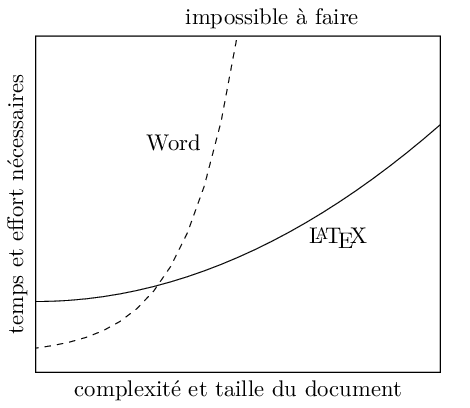
\includegraphics[scale=0.6]{Images/latex_word.png}
  \begin{tabular}{p{\textwidth}}
  Source: \cite{Peeters2013}
  \end{tabular}
\end{figure}

Enfin, avec RSweave on peut y intégrer des statisques que l'on a produit avec R sans faire de copier-coller et d'aller-retour entre plusieurs logiciels. Plus globalement, la construction de documents est facilitée: la révision voire le travail collaboratif peut se faire avec l'utilisation de Git qui est intégrée à Rstudio notamment.

C'est donc pour ces raisons que je vous présente aujourd'hui cette petite introduction à \LaTeX. Nous verrons dans un premier temps quels sont les notions de base du langage, avant de s'attarder sur les commandes principales puis nous verrons comment cela s'adapte à un document RSweave, c'est-à-dire en lien avec R.

\section{Les principes de base de \LaTeX}
\subsection{Installation}
\subsubsection{Windows}
Le plus simple est de télécharger Mik\TeX. Cependant, j'ai eu pas mal de soucis de compatibilité sur Windows, notamment avec RSweave. N'étant pas fan de Windows, j'ai préféré opter pour une solution que j'avais sur MacOS et sur Linux: \TeX Live. Vous le trouverez \href{https://tug.org/texlive/quickinstall.html}{ici} mais il vous faudra peut-être télécharger à part l'ISO pour éviter les échecs de téléchargement via l'installateur rapide. Toute la manipulation est expliquée \href{https://tug.org/texlive/doc/texlive-en/texlive-en.html#installation}{là}.

\subsubsection{MacOS}
Le plus simple cette fois est de directement télécharger \TeX Live. Tout le nécessaire vient avec sans complication. Voici le lien correspondant: \href{http://www.tug.org/mactex/}{http://www.tug.org/mactex/}.

\subsubsection{Linux}
Sous Linux, il suffit de faire la commande suivante dans le terminal:
\begin{minted}[bgcolor=bg]{shell}
sudo apt-get install texlive-full
\end{minted}

\subsection{Notion de compilation}
On l'a vu, \LaTeX{} ne permet pas de visualiser le résultat en direct, ce qui fait que l'on doit compiler pour voir ce que ça donne. On a un peu simplifié en disant qu'il n'y avait qu'une seule compilation, en effet selon la complexité du document on peut en avoir plusieurs. Le cas le plus typique est celui des références internes au document (bibliographie, renvois vers une figure comme ici: \ref{exemple_ref}). On aura alors une première compilation pour obtenir un fichier \texttt{.aux} qui stocke les étiquettes (on peut créer des labels ou faire des appels à la bibliographie) que l'on a créées ainsi que les lignes dans lesquelles on les mentionne. Ensuite une deuxième compilation est lancée en prenant en compte le fichier \texttt{.aux}, ce qui ajoute les liens hypertextes si besoin mais surtout numérote les références correctement. Ainsi, \LaTeX{} ne peut pas se tromper en numérotant une classe d'objet puisqu'il référence toutes les objets et les numérote sauf indication contraire.


\begin{figure}[h!]
  \caption{Schéma explicatif de la compilation}
  \label{compilation}
  \centering
  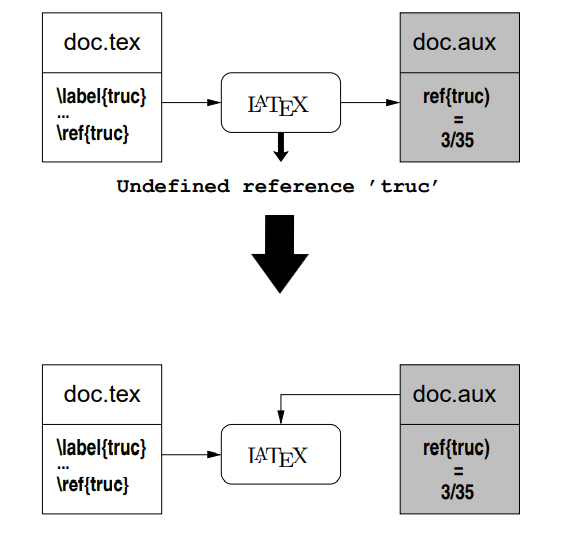
\includegraphics[scale=0.6]{Images/compilation.png}
  \begin{tabular}{p{\textwidth}}
  Source: \cite{Lozano2008}
  \end{tabular}
\end{figure}

En cas d'apparition de la table des matières, le processus est le même mais avec un fichier \texttt{.toc} et pour la bibliographie, une compilation de plus avec \texttt{biber} ou \texttt{Bib\LaTeX} produit un fichier \texttt{.bbl}.

\subsection{Notions principales}
\subsubsection{Packages}
Si vous êtes familiers avec R, la notion de package ne vous est pas étrangère. Dans le langage \LaTeX{}, on a la même logique: chaque fonction est définie dans un package que l'on se doit d'appeler avant d'appeler la fonction. En effet, cela demanderait bien trop de mémoire de charger l'ensemble des fonctions existantes dans la documentation. Cependant, d'expérience, la documentation et les ressources sur les forums sont bien plus nombreux, détaillés et accessibles! Ce qu'il est important de noter donc, c'est que si vous voulez réaliser quelque chose alors quelqu'un l'aura très probablement fait avant vous et il vous suffira de charger le package et donc les fonctions désirées. Dans le pire des cas, vous créerez une macro à partir d'une fonction existante.

\subsubsection{Préambule}
Contrairement à R  où l'on fait ce qu'on veut, on appelle les packages dans le préambule du fichier \texttt{.tex}, c'est-à-dire à l'extérieur de notre environnement de texte -- on y reviendra. On aura ainsi comme modèle de fichier \texttt{.tex} par défaut, un code impérativement délimité comme suit:
\begin{minted}[bgcolor=bg]{tex}
% Les commentaires sont indiques par un pourcentage
% On se trouve ici dans le preambule
\documentclass{article} % la classe de document est obligatoire, elle permet à LaTeX de charger des styles par defaut. Ici j'ai choisi article mais cela peut etre report, memoir, book, letter, ou bien d'autres
% On peut aussi creer sa propre classe

\usepackage{package1} % J'appelle ici package1, on verra plus tard lesquels peuvent nous être utiles

\begin{document}
% Ici on ne se trouve plus dans le preambule. L'ensemble de ce qui apparait dans le PDF se trouve la.
\end{document}
\end{minted}

\subsubsection{Classe}
Comme mentionné plus haut, j'ai utilisé ici la classe de documents \texttt{article}. Celle-ci répond à certains critères notamment en terme de structure de document. On dénombre sept niveaux de titres au total:
\begin{table}[!ht]
  \centering
  \begin{tabular}{|l|l|c|}
  \hline Commande & Sens & Niveau\\
  \hline \nomfonction{part} & Partie & $-1$\\
  \nomfonction{chapter} & Chapitre & $0$\\
  \nomfonction{section} & Section & $1$\\
  \nomfonction{subsection} & Sous-section & $2$\\
  \nomfonction{subsubsection} & Sous-sous-section & $3$\\
  \nomfonction{paragraph} & Paragraphe & $4$\\
  \nomfonction{subparagraph} & Sous-paragraphe & $5$\\
  \hline
  \end{tabular}
\end{table}

A titre d'exemple, la classe \texttt{article} ne commence qu'au niveau 1 alors que \texttt{book} commence au $-1$. Pour vous faire une idée, ce document utilise cette classe.

Voici quelques exemples de classes:
\begin{itemize}
  \item \texttt{article}: pour des textes relativement cours comme des articles scientifiques;
  \item \texttt{report}: pour des documents longs de plusieurs chapitres;
  \item \texttt{book}: pour des livres de plusieurs centaines de pages;
  \item \texttt{memoir}: pour écrire des mémoires (c'est ce que j'ai utilisé pour le mien, mais \texttt{report} semble également pertinent)
\end{itemize}

\subsection{Environnement}
Un environnement est un espace délimité dans lequel certaines règles précises et certaines fonctions ont cours. Il permet de créer ou d'importer des objets qui se définissent eux-mêmes comme des environnement aussi. L'environnement le plus utilisé est, logiquement \texttt{document} que l'on vient de voir. Il est obligatoire pour créer un document. Pour comprendre un peu mieux, prenons l'environnement \texttt{equation}. Dans celui-ci, les outils mathématiques -- contenus dans le package \texttt{amsmaths} -- ont un sens et n'en ont aucun en dehors. Voici un exemple:

\begin{minted}[bgcolor=bg]{tex}
\documentclass{article}
\usepackage{amsmaths}

\begin{document}
  \begin{equation}
  f(x)=\sqrt{x} % racine carrée
  \end{equation}
\end{document}
\end{minted}

Cela donne:
  \begin{equation}
  f(x)=\sqrt{x} % racine carrée
  \end{equation}
une équation numérotée basique.

Certains environnements sont appelés \emph{flottants} car ils ne font pas partie du texte et sont placés par \LaTeX{} là où cela est le plus optimal possible compte tenu du texte au-dessus et en-dessous, on verra plus bas qu'il s'agit surtout des tableaux et figures.

\section{Construction d'un document \LaTeX}
Nous pouvons maintenant passer à une partie un peu plus pratique.

\subsection{Choix courants dans le préambule}
Dans le préambule, on renseigne également le nom de l'auteur, le titre et la date. Le code du document présent comporte les commandes suivantes:

\begin{minted}[bgcolor=bg]{tex}
\documentclass[a4paper, 11pt]{article} % entre crochet on peut integrer des options a la commande de classe du document mais aussi aux packages
\usepackage{hyperref} % pour les liens hypertextes, ici cela ajoute le lien pour m'envoyer un mail
\usepackage{titling} % pour le titre en gras
\author{\href{mailto:julioricardo.davalos@ehess.fr}{Julio Ricardo Davalos}}
\title{Petite introduction à \LaTeX{} en Sciences Sociales}
\date{Septembre 2022}

% packages
\begin{document}
    \maketitle
%%%% La suite
\end{document}
\end{minted}

Le titre apparaît alors comme vous pouvez le voir plus haut, avec la date de dernière compilation en mode par défaut. Si je veux forcer une date, je fais comme dans l'exemple (il est possible de formater la commande pour qu'elle ne dise pas le jour, mais c'est tout aussi simple pour notre niveau).

\subsection{Environnements et packages usuels}
\subsubsection{Environnement \texttt{tabular} et ses dérivés}
Comme son nom l'indique, c'est un environnement qui sert à construire des tableaux. Il n'est pas flottant par défaut, ce qui fait qu'on le positionne généralement dans un flottant comme \texttt{table} ou \texttt{figure} si jamais on veut mettre une légende par exemple. Ces flottants prennent des arguments qui ont trait à leur position dans la page.

\begin{minted}[bgcolor=bg]{tex}
  \begin{table}[!ht] % permet de forcer la position "here top"
      \caption{Un tableau centré} % titre du table, ne marche que dans un flottant
      \centering % je centre dans la page
      \begin{tabular}{|c|c|} % 2 colonnes, texte centré, avec les lignes verticales tracées
      \hline %ligne horizontale
       Case $(1,1)$ & Case $(1,2)$ \\ %saut de ligne, "&" délimite une colonne
      \hline %ligne horizontale
      Case $(2,1)$ & Case $(2,2)$ \\ 
      \hline  %ligne horizontale
      \end{tabular}
  \end{table}
\end{minted}

Ce code donne:

  \begin{table}[!ht]
    \caption{Un tableau vide et centré}
    \centering
    \begin{tabular}{|c|c|}
    \hline 
    Case $(1,1)$ & Case $(1,2)$ \\ 
    \hline 
     Case $(2,1)$ & Case $(2,2)$ \\ 
    \hline 
    \end{tabular}
  \end{table}

Les arguments de base de \texttt{tabular} permettent de sélectionner le nombre de colonnes, leur alignement (\texttt{c}, \texttt{l} et \texttt{r}) et l'apparition des bordures par le symbole |. Les lignes de séparation des colonnes ne sont pas obligatoires, ainsi, on peut supprimer la ligne du milieu en indiquant \texttt{|cc|}. On peut construire autant de lignes et de colonnes que l'on veut, faire autant de \texttt{tabular} dans un \texttt{table} que l'on veut.

Evidemment cela est un peu fastidieux à écrire, mais beaucoup d'éditeurs existent, par exemple \href{https://www.latex-tables.com/}{ici}, mais aussi dans l'éditeur \TeX maker qui est plutôt pratique bien que moins adapté à R. Pour fusionner des cases, il faudra faire appel à la fonction \texttt{multicolumn} et \nomfonction{multirow} (cette dernière, vient du package du même nom).

\subsubsection{Environnement \texttt{figure}}
Cet environnement est également essentiel car il permet d'ajouter des images, qu'elles soient en PDF ou en format image, voire produite par votre document, on le verra ensuite. Il nécessite le package \texttt{graphicx}.

\begin{minted}[bgcolor=bg]{tex}
\begin{figure}[!ht] % permet de forcer la position "here"
	\caption{Une image prise au hasard} % titre, bien placé dans un flottant
	\centering % on centre
	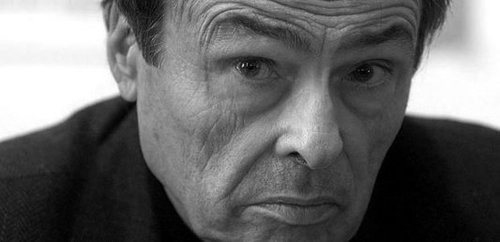
\includegraphics[scale=0.4]{Images/bourdieu.jpg} % insertion d'une image
	% taille = 40% de la largeur d'un paragraphe, on met le chemin de l'image
\end{figure}
\end{minted}

La ligne 4 peut être utilisée toute seule pour insérer une image tout comme \texttt{tabular} mais celle si sera placée là où \LaTeX{} calcule qu'elle a sa place optimale et elle n'aura pas de titre, donc il vaut mieux la garder dans un flottant. Ce code donne:

\begin{figure}[!ht]
	\caption{Une image choisie complètement au hasard}
	\centering
	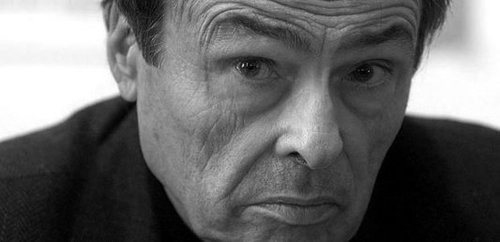
\includegraphics[scale=0.4]{Images/bourdieu.jpg}
\end{figure}


On peut également combiner les deux environnements en faisant des tableaux (avec ou sans lignes) contenant des images.

\subsubsection{Environnements \texttt{itemize} et \texttt{enumerate}}
Ces deux environnements sont très importants également car ils permettent de faire des listes. \texttt{itemize} permet de faire une suit de tirets (ou autre symbole que l'on choisit) et \texttt{enumerate}, une liste numérotée. Ils fonctionnent exactement de la même façon.

\begin{minted}[bgcolor=bg]{tex}
\begin{itemize}
  \item point 1
  \item point 2
\end{itemize}
\end{minted}

Ce code nous donne:
\begin{itemize}
  \item point 1
  \item point 2
\end{itemize}

On peut modifier les types de tirets ponctuellement en ajoutant ce que l'on veut entre crochets après la commande \nomfonction{item}

\subsubsection{Packages d'encoding et de typographie}
Les packages permettant d'écrire en français avec les bons accents et la typographie standard sont les suivants:
\begin{itemize}
\item \nomfonction[inputenc]{usepackage[utf8]}: permet à \LaTeX{} de comprendre l'encodage d'entrée, notamment pour les accents.
\item \nomfonction[babel]{usepackage[french]}: permet d'avoir les typographies françaises.
\item \nomfonction[fontenc]{usepackage[T1]}: permet d'encoder le PDF de sortie en T1.
\item \nomfonction[hyperref]{usepackage}: permet de créer des liens hyper-textes.
\item \nomfonction[geometry]{usepackage[left=cm,right=cm,top=cm,bottom=cm]}: permet de définir les marges.
\item \nomfonction[tabularx]{usepackage}: variante de \texttt{tabular} avec plus d'options.
\end{itemize}

\subsection{Corps du texte} 
Nous avons vu plus haut les commande pour la structuration des titres. Concernant la rédaction, il y a plusieurs choses à savoir:
\begin{itemize}
\item Plusieurs espaces à la suite produisent une seule espace.
\item Une ligne vide produit un changement de paragraphe. Plusieurs lignes vides produisent le même effet. Pour redémarrer avec l'indentation, on termine un paragraphe avec \textbackslash{}\textbackslash{}. Mais cette manière de faire n'est pas très propre, le mieux est de préciser dans le préambule quelle indentation on veut et quel espace entre les paragraphes on souhaite. Dans ce document j'ai simplement appelé le package \texttt{parskip} qui convient en version par défaut.
\item Un retour à la ligne est compris comme une espace.
\item Un espace \emph{après} un signe de ponctuation est obligatoire, mais \LaTeX{} comprend qu'il faut en faire un \emph{avant} et l'insèreun espace si besoin. Par ailleurs, il vaut mieux ne pas séparer la ponctuation du mot précédent, sans quoi \LaTeX{} risque de faire apparaître le signe sur la ligne suivante si le mot était le dernier de la ligne.
\item quatre caractères spéciaux ne s'obtiennent pas avec \textbackslash[mon caractère spécial]:
  \begin{enumerate}
  \item \textbackslash{} : qui s'insère avec \texttt{textbackslash};
  \item \textasciitilde{} : qui s'insère avec \texttt{textasciitilde};
  \item \textasciicircum{} : qui s'insère avec \texttt{textasciicircum}.
  \end{enumerate}
\item Les guillemets s'insèrent avec \nomfonction[mon texte]{enquote}.
\item L'italique s'obtient en insérant: \nomfonction[mon texte]{textit}.
\item Le gras s'obtient en insérant: \nomfonction[mon texte]{textbf}.
\end{itemize}

Enfin, dans le corps du texte on trouvera des liens hypertextes que l'on marque avec \nomfonction[mon label]{label} dans l'environnement auquel appartient le label puis que le pointe avec \nomfonction[mon label]{ref}.


\subsection{Bibliographie}
Pour ce qui est de la bibliographie, beaucoup de configurations existent et ce document n'a pas vocation à en donner une vue globale tant cela serait long. On peut également écarter la question de la création des fichiers \texttt{.bib} car ils sont aisément produits par Zotero par exemple. Un outil important à ajouter à ce dernier est l'extension BetterBib\LaTeX{} que l'on trouve \href{https://github.com/retorquere/zotero-better-bibtex/releases/tag/v6.7.23}{ici} et qui permet de standardiser ses sorties \texttt{.bib} et de les garder à jour. Ainsi, vos modifications dans Zotero se répliqueront dans le PDF final après re-compilation.

Une fois un fichier \texttt{.bib} joint au fichier \texttt{.tex}, on peut appeler le package \texttt{biblatex}. Pour une utilisation avec Rsweave, je recommande de mettre l'option \texttt{backend=biber} car ce processus fonctionne généralement mieux avec. Ensuite, selon vos préférences, vous pouvez régler les options selon votre style de citation favori. Zotero aura attribué une clé en fonction des préférences, par exemple \enquote{AuteurDate}, cette clé servira alors à appeler la ressource bibliographique ainsi:

\begin{minted}[bgcolor=bg]{tex}
 \cite{Rouquette2011}
\end{minted}

donne ici: 

\cite{Rouquette2011}. 

Je vous encourage d'ailleurs à aller voir la partie bibliographie de ce livre qui est particulièrement bien fournie et adaptée pour les SHS.


\section{Mise en forme de résultats statistiques avec \LaTeX}
Nous allons maintenant revenir à ce qui nous intéresse en tant qu'ingénieurs ou chercheurs: la publication. Pour produire des traitements statistiques, nous pouvons notamment utiliser R. RSweave permet de lier R et \LaTeX.

\subsection{Logique de RSweave}
\subsubsection{Interface}
RSweave est inclu dans Rstudio. On le trouve comme sur l'image qui suit:
\begin{figure}[!ht]
	\begin{center}
	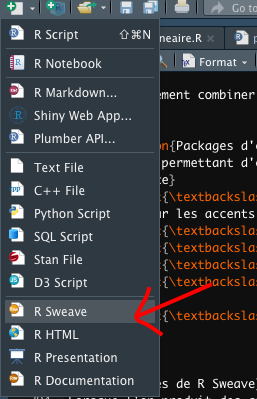
\includegraphics[width=0.25\textwidth]{Images/Sweave.png}
	\end{center}
\end{figure}
\newpage
Pour obtenir la version de Sweave la plus efficace et la plus documentée, il faut cependant sélection \texttt{knitr} (qui vient de Markdown), dans les paramètres. De même, comme vous avez installé \LaTeX{}, vous pouvez sélectionner pdf\LaTeX{} et oublier \texttt{tinytex} qui est une version légère de \LaTeX{}.
\begin{figure}[!ht]
	\begin{center}
	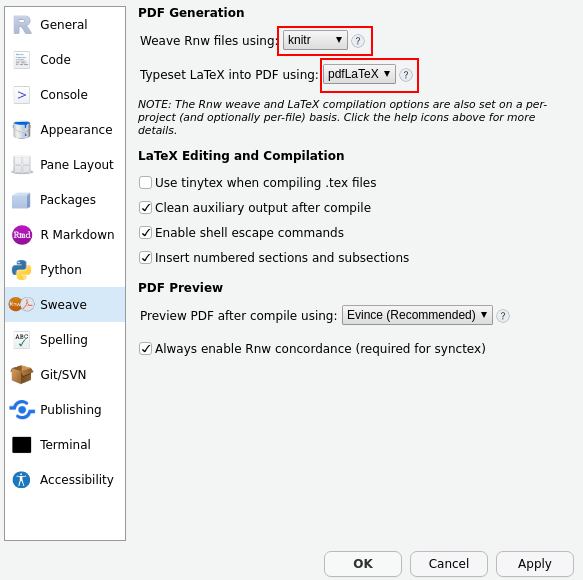
\includegraphics[width=0.4\textwidth]{Images/Options_Sweave.png}
	\end{center}
\end{figure}

\subsubsection{Notion de Chunk}
Le chunk est l'objet qui permet de faire le lien entre \LaTeX{} et R. Il s'insère dans un fichier \texttt{.Rnw} via le code suivant:
\begin{minted}[bgcolor=bg]{latex}
# <<>>=
print("une commande R")
@
\end{minted}
qui donne:
\begin{knitrout}
\definecolor{shadecolor}{rgb}{0.969, 0.969, 0.969}\color{fgcolor}\begin{kframe}
\begin{verbatim}
## [1] "une commande R"
\end{verbatim}
\end{kframe}
\end{knitrout}

\paragraph{NB:} ce fichier étant codé sur RSweave, j'ai dû ajouter des dièses pour qu'il ne prenne pas en compte le Chunk. Si quelqu'un a une solution pour réparer ça, j'en serais ravi.

Les chunks doivent comprendre toutes les commandes du code R dont on a besoin, y compris le chargement de répertoire, des bases de données etc. Il est possible d'en imprimer le contenu, la sortie ou les deux dans le PDF \LaTeX{}. Il dispose de différents arguments que l'on va utiliser ici:
\begin{itemize}
\item \texttt{eval=[T ou F]}: permet de lancer le code ou non. \textit{Sa valeur par défaut est \texttt{T}}.
\item \texttt{echo=[T ou F]}: permet d'imprimer ou non le code R contenu dans le chunk. \textit{Sa valeur par défaut est \texttt{T}}.
\item \texttt{fig=[T ou F]}: permet d'avoir une sortie de type figure ou non. Cela revient à faire \textbackslash{}includegraphics, il vaut donc mieux penser à ajouter un environnement \texttt{figure} autour comme on l'a vu plus haut, même si cela n'est pas absolument nécessaire. \textit{Sa valeur par défaut est \texttt{F}}.
\item \texttt{results=[verbatim, tex ou hide]}: permet d'afficher une sortie R paramétrée pour être au langage \LaTeX{} ou verbatim. On l'utilisera ici pour les \texttt{xtable}. \textit{Sa valeur par défaut est \texttt{hide}}.
\item \texttt{label=}: permet de donner un nom au chunk afin de potentiellement y faire appel plus tard.
\item \texttt{fig.width=} et \texttt{fig.height=}: permet de donner une taille à la sortie s'il s'agit d'une image (par exemple un graphique).
\end{itemize}

\subsubsection{Le hic: la bibliographie}
Il devait bien y avoir un hic dans cette histoire. Il s'agit de l'importation de la bibliographie. RStudio ne permet pas de lier \texttt{biber} à notre fichier de manière automatique. Cela implique qu'en théorie, on ne peut pas mettre de bibliographie dans un fichier Rsweave compilé depuis Rstudio. Deux solutions existent pour ce problème:
\begin{enumerate}
 \item Vous utilisez un autre compilateur, par exemple \TeX maker qui lui est modifiable et à qui on peut donc dire où sont les outils dont il a besoin pour réaliser chaque tâche. Un autre exemple est Emacs qui comprend énormément de langages et vous permettra de faire à peu près tout. Mais cette solution implique que l'on se passe de l'interface de Rstudio qui est pourtant très ergonomique et moins aride.
 \item Vous restez sur Rstudio et vous ajoutez en fin de document, le code suivant:
 \begin{minted}[bgcolor=bg]{R}
\end{document}
# <<setup, eval= TRUE, include= FALSE, cache= FALSE, echo= FALSE>>=
system (paste ("biber", sub ("\\.Rnw$", "", current_input())))
@
\end{minted}
\item[] cela va forcer \texttt{biber} à compiler le document. Il faudra cependant compiler deux fois à chaque fois que vous citez une nouvelle entrée bibliographique.
\end{enumerate}

\subsection{Exemples de tableaux}
On peut maintenant créer une base de données, je reprends ici une idée d'exemple reproductible que j'avais fait pour autre chose.

\begin{minted}[bgcolor=bg]{R}
# <<>>=
data <- data.frame(choix = sample(c("fraise", "mangue", "orange", "cerise"), 
                                  1000, replace = T, 
                                  prob = c(0.5, 0.2, 0.2, 0.1)),
                   aime_kiwi = sample(c("Oui", "Non"), 1000, 
                                      replace = T, prob = c(0.2, 0.8)),
                   aime_melon = sample(c("Oui", "Non"), 1000, 
                                      replace = T, prob = c(0.5, 0.5)),
                   aime_ananas =  sample(c("Oui", "Non"), 1000, 
                                      replace = T, prob = c(0.7, 0.3)))
@
\end{minted}


On veut les fréquences des \enquote{choix}, que l'on fait avec une fonction de base.
\begin{minted}[bgcolor=bg]{R}
# <<>>=
library(questionr)
freq(data$choix)
@
\end{minted}
\begin{knitrout}
\definecolor{shadecolor}{rgb}{0.969, 0.969, 0.969}\color{fgcolor}\begin{kframe}
\begin{verbatim}
##          n    % val%
## cerise  25  8.3  8.3
## fraise 158 52.7 52.7
## mangue  49 16.3 16.3
## orange  68 22.7 22.7
\end{verbatim}
\end{kframe}
\end{knitrout}

Le résultat n'est pas satisfaisant. Avec le package \texttt{kableExtra}, on peut faire bien mieux:
\begin{minted}[bgcolor=bg]{R}
# <<result="asis">>=
# result="asis" permet de dire à Sweave que le Chunk va contenir du texte
library(kableExtra)
library(tidyverse)
freq(data$choix) %>% 
 kable(format = "latex", # sinon c'est en html
       caption = "Fréquence des choix",
       label = "freqchoix",
       booktabs = TRUE) %>%  # permet d'avoir des tableaux plus jolis, necessite le package booktabs dans le preambule
    kable_styling(latex_options = c("hold_position"), # cree un float et lui donne l'argument 'h'
                  position = "center") # centre le tableau
@
\end{minted}
\begin{knitrout}
\definecolor{shadecolor}{rgb}{0.969, 0.969, 0.969}\color{fgcolor}\begin{table}[!h]

\caption{\label{tab:freqchoix}Fréquence des choix}
\centering
\begin{tabular}[t]{lrrr}
\toprule
  & n & \% & val\%\\
\midrule
cerise & 25 & 8.3 & 8.3\\
fraise & 158 & 52.7 & 52.7\\
mangue & 49 & 16.3 & 16.3\\
orange & 68 & 22.7 & 22.7\\
\bottomrule
\end{tabular}
\end{table}

\end{knitrout}

Ce package permet de prendre en compte beaucoup de paramètres dans les tableaux. Par exemple, on peut les mettre sur une page unique, en format paysage, avec des cases de couleur etc. Je ne peux que vous recommander la lecture de sa documentation \href{https://haozhu233.github.io/kableExtra/}{ici}. A partir de maintenant, je ne mettrai plus que les codes de R grâce à l'argument \texttt{echo=T} et non plus le chunk en entier.

Pour le cas des tableaux de régression, un package dédié et très connu a été développé: \texttt{stargazer}. Imaginons que l'on veuille faire des modèles de régression dans le rendu

\begin{kframe}
\begin{alltt}
\hlkwd{library}\hlstd{(glm2)}
\hlstd{data} \hlkwb{<-} \hlstd{data} \hlopt
 \hlkwd{mutate}\hlstd{(}\hlkwc{choix_fraise} \hlstd{=} \hlkwd{case_when}\hlstd{(choix} \hlopt{==} \hlstr{"fraise"} \hlopt{~} \hlstr{"Oui"}\hlstd{,} \hlnum{TRUE} \hlopt{~} \hlstr{"Non"}\hlstd{)} \hlopt
         \hlkwd{as.factor}\hlstd{(),}
        \hlkwc{choix_cerise} \hlstd{=} \hlkwd{case_when}\hlstd{(choix} \hlopt{==} \hlstr{"cerise"} \hlopt{~} \hlstr{"Oui"}\hlstd{,} \hlnum{TRUE} \hlopt{~} \hlstr{"Non"}\hlstd{)} \hlopt
         \hlkwd{as.factor}\hlstd{(),}
        \hlkwc{age} \hlstd{=} \hlkwd{sample.int}\hlstd{(}\hlnum{100}\hlstd{,} \hlnum{1000}\hlstd{,} \hlkwc{replace} \hlstd{= T),}
        \hlkwc{nb_fruits} \hlstd{= (aime_kiwi} \hlopt{==} \hlstr{"Oui"}\hlstd{)} \hlopt{+} \hlstd{(aime_melon} \hlopt{==} \hlstr{"Oui"}\hlstd{)} \hlopt{+}
         \hlstd{(aime_ananas} \hlopt{==} \hlstr{"Oui"}\hlstd{)} \hlopt{+} \hlkwd{abs}\hlstd{(}\hlkwd{rnorm}\hlstd{(}\hlnum{1000}\hlstd{,} \hlkwc{mean} \hlstd{=} \hlkwd{log}\hlstd{(age))))}
\hlcom{# j'ai ajouté un bruit aléatoire en fonction de l'âge exprès}

\hlstd{m1} \hlkwb{<-} \hlkwd{glm}\hlstd{(choix_fraise} \hlopt{~} \hlstd{age} \hlopt{+} \hlstd{aime_kiwi} \hlopt{+} \hlstd{aime_melon} \hlopt{+} \hlstd{aime_ananas,}
          \hlkwc{family} \hlstd{= binomial,} \hlkwc{data} \hlstd{= data)}
\hlstd{m2} \hlkwb{<-} \hlkwd{glm}\hlstd{(choix_cerise} \hlopt{~} \hlstd{age} \hlopt{+} \hlstd{aime_kiwi} \hlopt{+} \hlstd{aime_melon} \hlopt{+} \hlstd{aime_ananas,}
          \hlkwc{family} \hlstd{= binomial,} \hlkwc{data} \hlstd{= data)}
\hlstd{m3} \hlkwb{<-} \hlkwd{lm}\hlstd{(nb_fruits} \hlopt{~} \hlstd{age} \hlopt{+} \hlstd{aime_kiwi} \hlopt{+} \hlstd{aime_melon} \hlopt{+} \hlstd{aime_ananas,} \hlkwc{data} \hlstd{= data)}

\hlkwd{library}\hlstd{(stargazer)}
\hlkwd{stargazer}\hlstd{(m1,m2, m3,} \hlkwc{title} \hlstd{=} \hlstr{"Trois beaux modèles"}\hlstd{)}
\end{alltt}
\end{kframe}
% Table created by stargazer v.5.2.3 by Marek Hlavac, Social Policy Institute. E-mail: marek.hlavac at gmail.com
% Date and time: mar., sept. 06, 2022 - 23:36:15
\begin{table}[!htbp] \centering 
  \caption{Trois beaux modèles} 
  \label{} 
\begin{tabular}{@{\extracolsep{5pt}}lccc} 
\\[-1.8ex]\hline 
\hline \\[-1.8ex] 
 & \multicolumn{3}{c}{\textit{Dependent variable:}} \\ 
\cline{2-4} 
\\[-1.8ex] & choix\_fraise & choix\_cerise & nb\_fruits \\ 
\\[-1.8ex] & \textit{logistic} & \textit{logistic} & \textit{OLS} \\ 
\\[-1.8ex] & (1) & (2) & (3)\\ 
\hline \\[-1.8ex] 
 age & $-$0.004 & 0.011$^{***}$ & 0.027$^{***}$ \\ 
  & (0.002) & (0.004) & (0.001) \\ 
  & & & \\ 
 aime\_kiwiOui & 0.037 & $-$0.358 & 0.978$^{***}$ \\ 
  & (0.157) & (0.297) & (0.083) \\ 
  & & & \\ 
 aime\_melonOui & $-$0.081 & $-$0.011 & 0.947$^{***}$ \\ 
  & (0.127) & (0.222) & (0.067) \\ 
  & & & \\ 
 aime\_ananasOui & 0.004 & $-$0.088 & 0.955$^{***}$ \\ 
  & (0.137) & (0.234) & (0.072) \\ 
  & & & \\ 
 Constant & 0.191 & $-$2.791$^{***}$ & 2.333$^{***}$ \\ 
  & (0.178) & (0.327) & (0.094) \\ 
  & & & \\ 
\hline \\[-1.8ex] 
Observations & 1,000 & 1,000 & 1,000 \\ 
R$^{2}$ &  &  & 0.524 \\ 
Adjusted R$^{2}$ &  &  & 0.522 \\ 
Log Likelihood & $-$691.623 & $-$302.110 &  \\ 
Akaike Inf. Crit. & 1,393.246 & 614.221 &  \\ 
Residual Std. Error &  &  & 1.057 (df = 995) \\ 
F Statistic &  &  & 273.853$^{***}$ (df = 4; 995) \\ 
\hline 
\hline \\[-1.8ex] 
\textit{Note:}  & \multicolumn{3}{r}{$^{*}$p$<$0.1; $^{**}$p$<$0.05; $^{***}$p$<$0.01} \\ 
\end{tabular} 
\end{table} 


Là encore, la fonction permet énormément de choses, beaucoup d'arguments sont utilisables ensemble. On peut notamment changer les noms des variables, ajouter des en-têtes, changer les coefficients par exemple pour des odds-ratio, calculer des statistiques d'ajustement etc. Des styles propres à des revues scientifiques sont pré-enregistrés dans la fonction pour faciliter son utilisation.

\subsection{Exemple de figure}
Pour les figures, cela est très facile également. Essayons avec un graphique.

\begin{knitrout}
\definecolor{shadecolor}{rgb}{0.969, 0.969, 0.969}\color{fgcolor}\begin{kframe}
\begin{alltt}
\hlcom{# dans les arguments du chunk, on a mis:}
\hlcom{# fig.cap="Nombre de fruits estimés en fonction de l'âge"}
\hlcom{# fig.lp="nbfruits_age" # (label)}
\hlcom{# fig.pos="ht!"}
\hlcom{# fig.width=7}
\hlcom{# fig.height=3}
\hlcom{# fig.env="figure"}
\hlcom{# echo=T}

\hlkwd{library}\hlstd{(ggplot2)}
\hlstd{data} \hlopt
 \hlkwd{ggplot}\hlstd{(}\hlkwd{aes}\hlstd{(}\hlkwc{x} \hlstd{= age,} \hlkwc{y} \hlstd{= nb_fruits))} \hlopt{+}
 \hlkwd{geom_point}\hlstd{()} \hlopt{+}
 \hlkwd{stat_summary}\hlstd{(}\hlkwc{fun.data} \hlstd{= mean_cl_normal)} \hlopt{+}
 \hlkwd{geom_smooth}\hlstd{(}\hlkwc{method}\hlstd{=}\hlstr{'lm'}\hlstd{)}
\end{alltt}
\end{kframe}\begin{figure}[ht!]
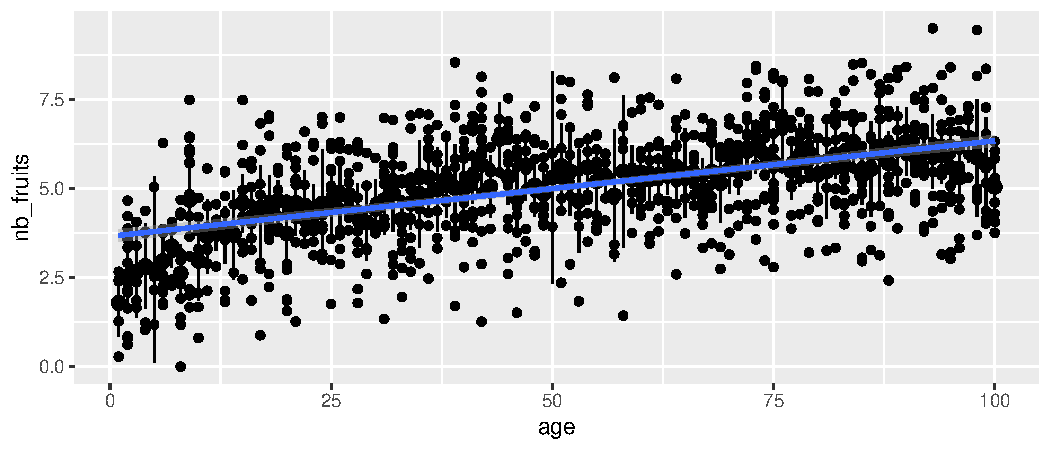
\includegraphics[width=\maxwidth]{Sorties/Graphunnamed-chunk-7-1} \caption[Nombre de fruits estimés en fonction de l'âge]{Nombre de fruits estimés en fonction de l'âge}\label{nbfruits_ageunnamed-chunk-7}
\end{figure}

\end{knitrout}

Pour plus d'options dans les chunk: \url{https://yihui.org/knitr/options/#chunk-options}.

\nocite{*}
\printbibliography
\end{document}

